\chapter{Diagrama de implementação}
\addcontentsline{toc}{chapter}{Diagrama de implementação}

A seguir o diagrama de implementação do sistema, que descreve a forma como os componentes de hardware e software interagem entre si.

\begin{figure}[H]
    \label{figure_diagrama_implementacao}
    \centering
    \caption{Diagrama de implementação}
    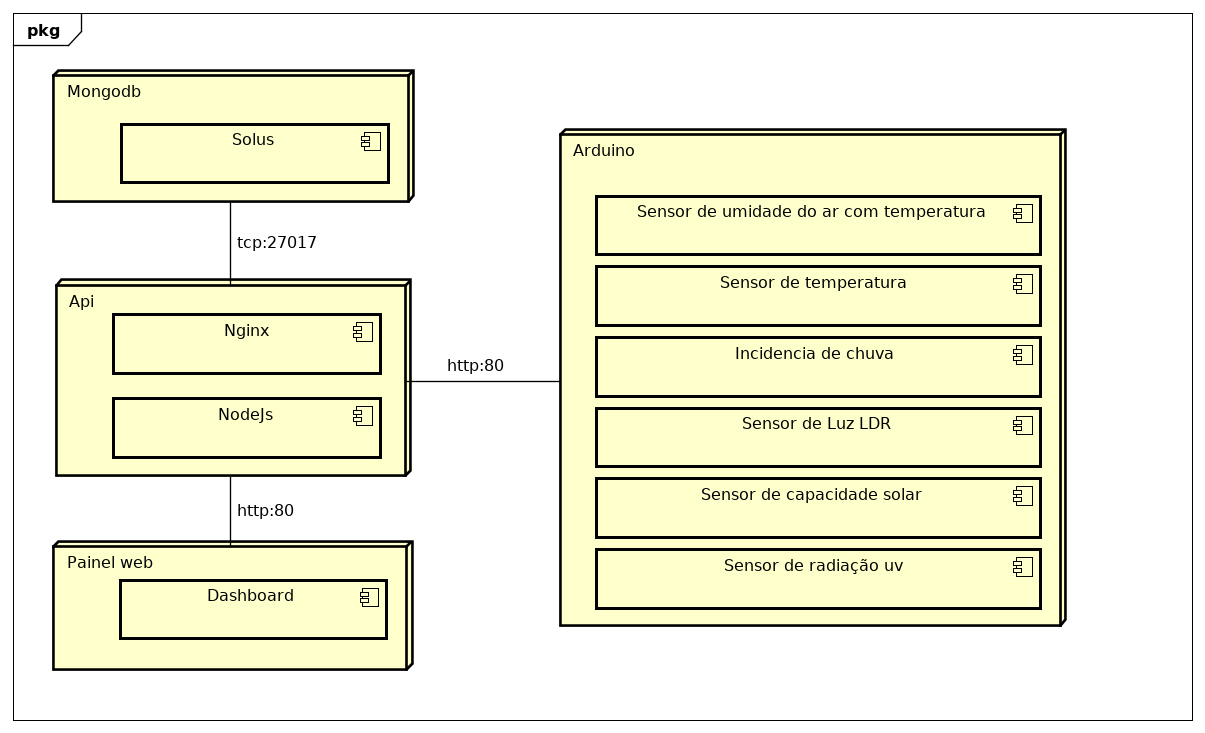
\includegraphics[scale=0.6]{diagrams/implementacao.png}
    \hfill
\end{figure}

\section{Sensores}

Os sensores do arduino, são ligados através da protoboard até o arduino, onde a captação é feita e as informações são tratadas, os dados são montados dentro de uma string JSON, que é enviada para o nodeMCU.

Não foi utilizada a biblioteca para a montagem da string JSON por conta da memória limitada do controlador.

\section{NodeMCU}

Na placa de WiFi NodeMCU, as informações são recebidas através da porta serial e o json recebido é enviado para a api.
